% Rebuild: pdflatex -output-directory=<build> weighted-conway-tree.tex
% SVG/PNG are direct page exports of that PDF (PyMuPDF get_svg_image/get_pixmap).
\documentclass[tikz,border=12pt]{standalone}
\usepackage[T1]{fontenc}
\usepackage{lmodern,amsmath}
\usetikzlibrary{arrows.meta}
\definecolor{ink}{HTML}{183444}
\definecolor{blue}{HTML}{1B6780}
\definecolor{amber}{HTML}{AD601A}
\begin{document}
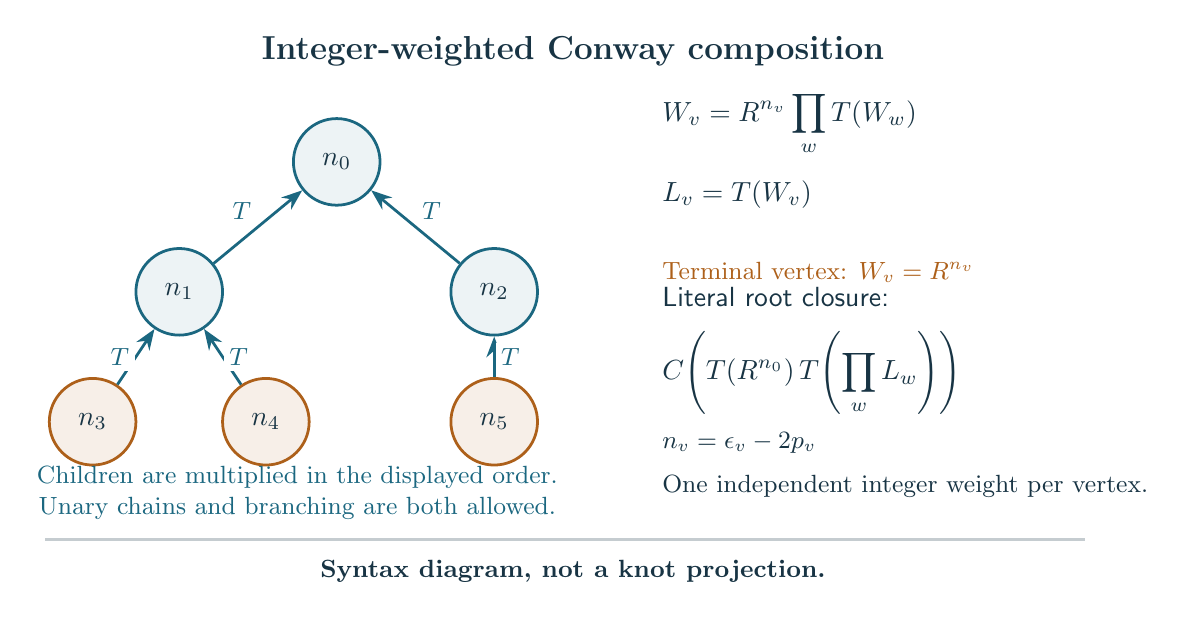
\begin{tikzpicture}[font=\sffamily,text=ink,line width=1pt,
  >=Stealth,
  weighted/.style={circle,draw=blue,fill=blue!8,minimum size=11mm},
  terminal/.style={weighted,draw=amber,fill=amber!10},
  turn/.style={font=\small,fill=white,inner sep=2pt,text=blue}]
 \node[font=\large\bfseries] at (0,3.5)
   {Integer-weighted Conway composition};
 \node[weighted] (v0) at (-3,2.1) {$n_0$};
 \node[weighted] (v1) at (-5,.45) {$n_1$};
 \node[weighted] (v2) at (-1,.45) {$n_2$};
 \node[terminal] (v3) at (-6.1,-1.2) {$n_3$};
 \node[terminal] (v4) at (-3.9,-1.2) {$n_4$};
 \node[terminal] (v5) at (-1,-1.2) {$n_5$};
 \draw[blue,->] (v1)--node[turn,above left]{$T$}(v0);
 \draw[blue,->] (v2)--node[turn,above right]{$T$}(v0);
 \draw[blue,->] (v3)--node[turn,left]{$T$}(v1);
 \draw[blue,->] (v4)--node[turn,right]{$T$}(v1);
 \draw[blue,->] (v5)--node[turn,right]{$T$}(v2);
 \node[font=\small,align=center,text=blue] at (-3.5,-2.1)
  {Children are multiplied in the displayed order.\\
   Unary chains and branching are both allowed.};
 \node[anchor=west,align=left] at (1,2.25)
  {$\displaystyle W_v=R^{n_v}\prod_w T(W_w)$\\[8pt]
   $\displaystyle L_v=T(W_v)$};
 \node[anchor=west,align=left,font=\small,text=amber] at (1,.7)
  {Terminal vertex: $W_v=R^{n_v}$};
 \node[anchor=west,align=left] at (1,-.3)
  {Literal root closure:\\[8pt]
   $\displaystyle C\!\left(T(R^{n_0})\,
             T\!\left(\prod_w L_w\right)\right)$};
 \node[anchor=west,align=left,font=\small] at (1,-1.75)
  {$n_v=\epsilon_v-2p_v$\\[5pt]
   One independent integer weight per vertex.};
 \draw[ink!25] (-6.7,-2.7)--(6.5,-2.7);
 \node[font=\small\bfseries,align=center] at (0,-3.1)
  {Syntax diagram, not a knot projection.};
\end{tikzpicture}
\end{document}
